\section{A3-E}\label{sec:A3-E}

\begin{figure}[tbp]
	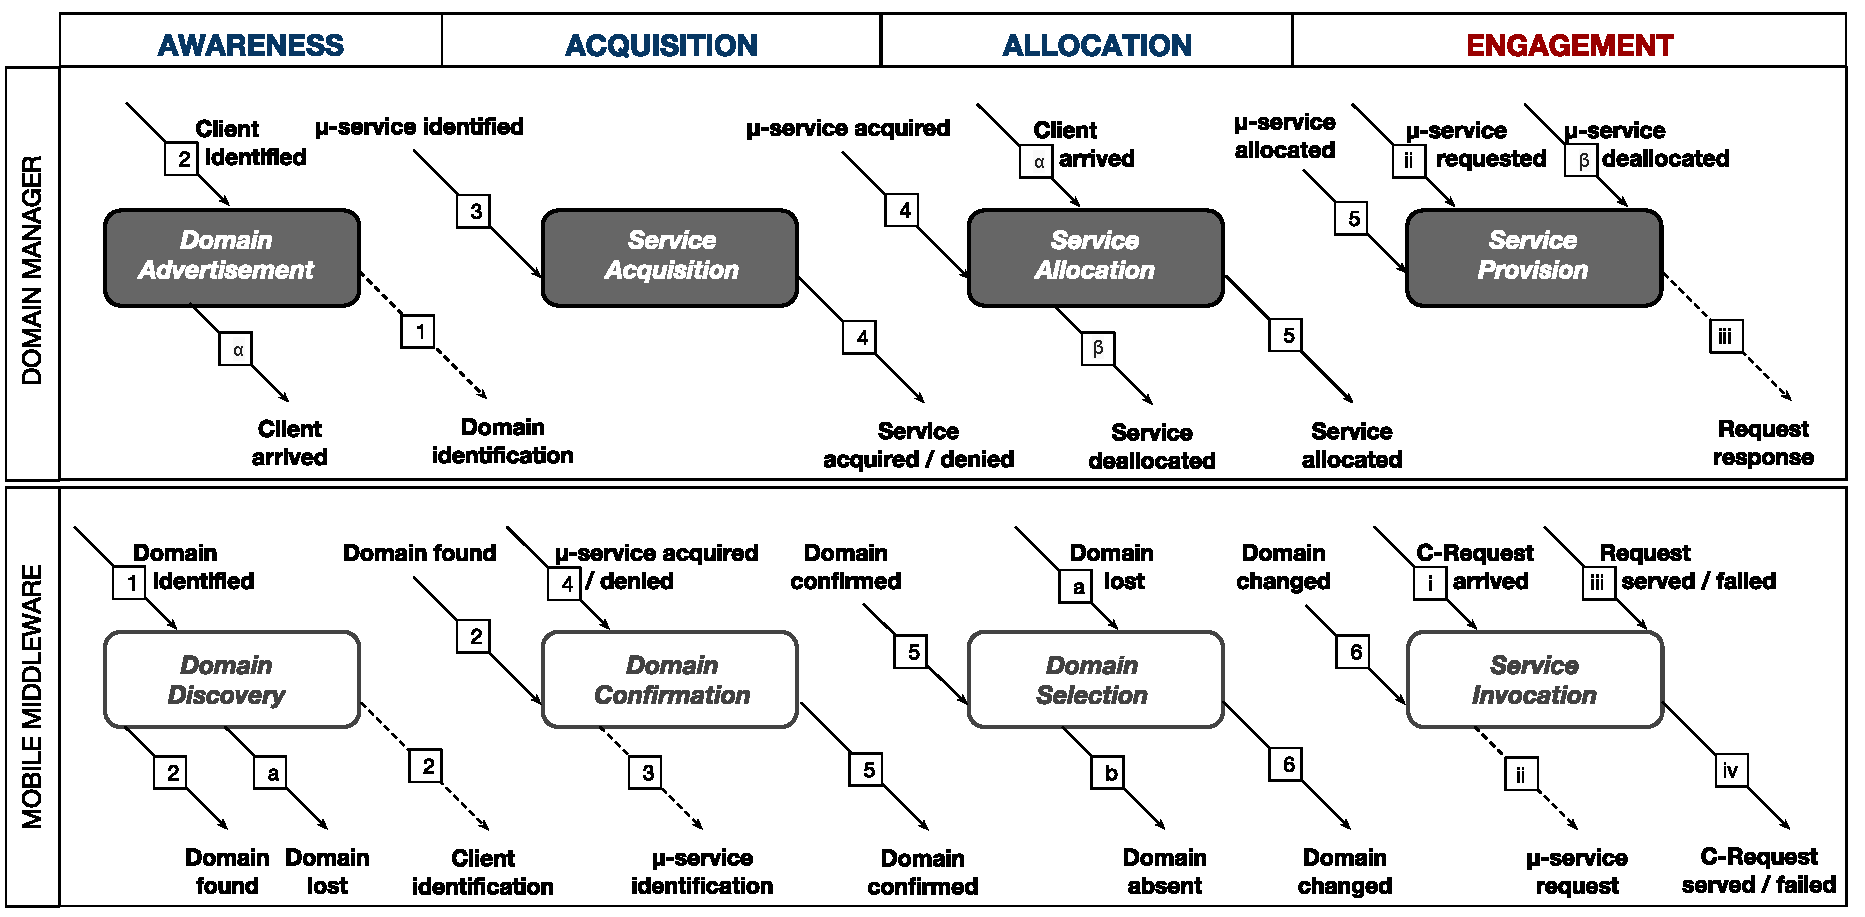
\includegraphics[width=1\textwidth]{figs/A3-E-process}
	\caption{A3-E overview. A3-E's activities are carried out by a \textit{domain manager} and a \textit{mobile middleware}; activities are coordinated through signals (dashed arrows) and events (solid arrows).}
	\label{fig:A3-E-process}
\end{figure}


%First and foremost, A3-E's main objective is to enable the efficient and scalable placement of $\mu$-services along the continuum. In A3-E, clients and providers autonomously interact and decide for the placement of services according to the context. Moreover,  

To realize the compute continuum, we propose A3-E
, a model supporting the self-management of continuum $\mu$-service life-cycle. A3-E inherits its name from its four main activities -- namely, \textit{(\textbf{A}wareness), (\textbf{A})cquisition, (\textbf{A})llocation, and (\textbf{E})ngagement}. 

%To realize the compute continuum, we propose A3-E, a model supporting the self-management of continuum $\mu$-services life-cycle. A3-E inherits its name from its four main activities -- namely, \textit{(\textbf{A}wareness), (\textbf{A})cquisition, (\textbf{A})llocation, and (\textbf{E})ngagement}. Clients and distinct providers (domains) take part in the \textit{automated} and \textit{decentralized} runtime decision of which continuum resources --- among those of mobile, edge, and cloud --- should be employed in the provisioning of each $\mu$-service required by continuum applications.

A3-E targets the efficient and scalable placement of $\mu$-services along the continuum. For this, clients and distinct providers (domains) take part in the \textit{automated} and \textit{decentralized} runtime decision of which continuum resources --- among those of mobile, edge, and cloud --- should be employed in the provisioning of each $\mu$-services required by continuum applications.

Figure~\ref{fig:A3-E-process} illustrates each activity in A3-E. The latter are refined by specific activities carried out by a \textit{domain manager} and by a \textit{mobile middleware}. These activities addresses different concerns in the interaction between client applications and continuum domains. 
%Activities from both sides are coordinated through signals and events. 
To address the intrinsic heterogeneity of the continuum, A3-E is flexible with respect to how each activity is employed.
%For each phase, the main activities of a \textit{domain} and a \textit{client} are depicted along with their mutual relative state at the moment the phase starts: for a domain, a service state ranges from \textit{Free} to \textit{Allocated}, whilst a domain state ranges from \textit{Away} to \textit{Selected} for a client. 
%More precisely, Fig.~\ref{fig:A3-E-process} refers to the activities and states (in parenthesis) of a single client-domain interaction.

%Next, we detail each main activity in A3-E, starting from the most general one, i.e., the one that applies to all types of client-domain interaction, and moving towards the more specific ones.


%\subsection{A3-E Process: Phases}\label{sec:A3-E-process}

%Next, the four A3-E phases are further described and mapped to the requirements elicited in  Section~\ref{sec:requirements}. Later on, other possible instances of the A3-E model are correlated with scenarios of the compute continuum.


\subsection{Awareness}\label{sec:A3-E-awareness}

From the provider's viewpoint, Awareness models the advertisement of domains and the discovery of continuum applications in one of its domains' coverage area, indicating the imminent need for the corresponding $\mu$-services. 

%Its main purpose is to enable domains to pro-actively initialize the Acquisition and Allocation activities, based on the awareness of devices in a domain's coverage area. 

Cloud domains are not likely to change, 
%known beforehand 
and may be set-up statically by clients.
Conversely, to achieve Awareness edge domains must advertise their existence (\textit{domain identification} signal) using discovery protocols compatible with its network infrastructure: for instance, through broadcasting in local-edge and control channels in mobile-edge~\cite{ETSI:MEC:ARCHITECTURE}. 
Upon a \textit{client identified} event, the domain manager must trigger both \textit{client arrived} and \textit{$\mu$-service identified} events for each required $\mu$-service.

%TODO this is a central problem tackled by A3-E and belongs to intro or wherever we discuss the problem
FaaS platforms like AWS Lambda~\cite{AWSLambda}
%~\footnote{https://docs.aws.amazon.com/lambda/latest/dg/running-lambda-code.html}
and OpenWhisk~\cite{OpenWhisk} adopt a cold start policy in which functions are allocated after their first call following a period of idleness. This latency, however, may be disruptive for some applications. In comparison, the proposed mutual client-provider awareness 
%Taking advantage of mutual client-provider awareness, the proposed mechanism 
has two benefits: (i) it alleviates the cold start by pro-actively allocating $\mu$-services just before they are needed; and (ii) it enables $\mu$-service acquisition to be opportunistic (i.e., on demand) by triggering the download and installation of $\mu$-services as soon as the client of a new application becomes active in that domain (e.g., by entering an edge domain's area).

%Throughout Awareness, the domain manager handles the following event:

%{\small
%\begin{itemize}
%	
%	\item \textbf{Client identified:} triggered when a new client enters the domain's coverage area. The manager must react with the triggering of a \textit{client arrived} and \textit{$\mu$-service identified} events for each $\mu$-service required by the client.
%	
%\end{itemize}
%}%




From the client's perspective, Awareness corresponds to the discovery of domains followed by a \textit{client identification} signal. More precisely, a \textit{client identification} must contain the $\mu$-service identification along with the repository from where it can be fetched during A3-E's Acquisition. To realize it, the mobile middleware can rely on special purpose HTTP endpoints from cloud domains, whereas local-edge and mobile-edge domains can respectively rely on protocols from local area (e.g., UDP) and radio access networks (e.g., control channels). Finally, the middleware can communicate with its mobile domain via system-level signals (e.g., broadcast intents in Android platforms).

In our running example, the mobile-edge and local-edge domains must advertise their existence to our user's device, which in turn identifies the AR and Image Editing applications. The same holds for the hotel's local-edge and the MG application. In all cases, cloud and edge domains can employ Awareness to opportunistically fetch, install, and allocate instances of required $\mu$-services.


%The mobile middleware, in turn, realizes Awareness with the discovery of cloud and edge domains. In particular, 
%During Awareness, the mobile middleware handles the following event:
%
%{\small
%\begin{itemize}
%	
%	\item \textbf{Domain identified:} triggered when a domain is found. The middleware must react with the triggering of a \textit{domain found} event and a \textit{client identification} signal to the domain manager.
%	
%\end{itemize}
%}%

%To implement Awareness, 

%It copes with the need for efficiency and scalability of finely distributed edge domains by allowing acquisition and/or allocation of services to happen just in time, i.e., just before the client application needs them.
%and enables not only functions to be allocated, but also acquired in an opportunistic fashion.
%The benefit lies in the anticipation of (opportunistic) services setup with respect to the arrival of the first service request, i.e., in the mitigation of service setup delay (also known as cold start). Since cloud domains cover a large area, the later do not employ the awareness phase. Needless to say, mobile domains do not require awareness for sharing the same platform with client applications.

%TODO [Danilo] Commented-out in favor of a more abstract description in terms of events, as broadcasting is something local-edge specific
%The DSM achieves this by broadcasting its existence and by waiting for clients to pass along their requirements. In our running example this occurs when the user's domestic local-edge server becomes aware of the new mobile game that the user had just installed. 
%%nd the discovery of client applications along with their requirements (i.e., services). The later are passed to the following phase of acquisition.
%%then receive all client application requirements (i.e., services) as soon as the client's mobile device enters the domain's coverage area, and then pro-actively starting acquisition and allocation. 
%%For example, in the real-time translation application previously introduced, the service setup delay was mitigated by having the acquisition of the data and codebase composing the service to start as soon as the user entered the edge domain's coverage area.
%%For example, the setup of services required by the mobile multiplayer game application by the user's local-edge server follows the awareness of a new application.
%From the client's perspective, the awareness phase models the discovery of domains, and corresponding $\mu$-services, whose network addresses are not previously known. In particular, it tackles edge domains that are integrated with the local network infrastructures of buildings and public spaces. This modality contrasts with cloud which are accessed through DNS and traffic managers. Needless to say, the awareness phase is not considered by mobile domains. The CSM intercepts the provider's broadcast messages, and reacts by sending back its application requirements. This process should happen once, and in a timely fashion, upon connection to new networks to mitigate battery consumption. As an example, the local-edge server in our user's home is discovered when her mobile device connects to her domestic Wi-Fi network. 


%Once the domain is ready, this domain becomes an alternative for the provisioning of services required by the many applications (e.g., the mobile multiplayer game) hosted by the user's smartphone, tablet, and/or other of his IoT gadgets. 


%Finally, the Awareness phase has the following purposes: 1) to enable domains to pro-actively initialize the acquisition and allocation phases based on its awareness of applications whose hosting devices happens to be in the domain coverage area (Req.~\textbf{R2.3}); and 2) to enable clients to discover the address of local domains (Req.~\textbf{R2.2}).

%From the domains perspective, the awareness of clients presence in their coverage area allows a proactive download and installation of services artifacts (acquisition phase) and/or the allocation of services (allocation phase) potentially before a first request to that service arrives, alleviating the delay introduced by services setup.  From the clients perspective, the awareness phase increases the range of alternatives from the continuum that can be used to satisfy their requirements.

%Such behavior allows that are opportunistically acquired and/or allocated to mitigate their setup delay by triggering these phases upon awareness of client(s) in their coverage area.

%From the domain-side, the lack of awareness of clients in the domain coverage area prevents triggering the acquisition and subsequently allocation phases based on this event. From the client-side, the lack of awareness from surrounding domains prevents them to make the decision of which domains to use. In the later case, clients must rely on external components to reach servers (e.g., traffic managers and DNS servers).

\subsection{Acquisition}\label{sec:A3-E-acquisition}

The \textit{Acquisition} models the automated download and installation of continuum $\mu$-service artifacts and the confirmation of the domain's capability in providing that $\mu$-service. Its ultimate goal is to mitigate the use of domain resources before the $\mu$-service is actually needed, while also facilitating IT operations (Ops) for developers and administrators. 

Ops mitigation is particularly important in (finely distributed) edge domains, since the manual administration of a large number of $\mu$-services can prove cumbersome and expensive. Nevertheless, this can also prove useful for cloud domains. Indeed, to the best of our knowledge, current FaaS platforms only support uploading (pushing) functions through public interfaces. 

Acquisition is autonomously managed, therefore it allows $\mu$-services to be downloaded 
%(e.g., pulled from a repository) 
and installed on demand. To achieve it, a domain manager must fetch the corresponding assets (e.g., compiled classes and dependencies) from a repository upon the arrival of a \textit{$\mu$-service identified} event. Note that mobile domains are exempt of performing Allocation as local $\mu$-services are assumed to be downloaded and installed along with the client application.

% In addition to function sources, artifacts may comprise data and libraries needed by the service.

%Throughout Acquisition, the domain manager handles the following event:
%
%{\small
%\begin{itemize}
%	
%	\item \textbf{$\mu$-service identified:} indicates the request for deployment of a new $\mu$-service. The manager must proceed with the download and installation of the $\mu$-service, followed by the triggering of a \textit{service acquired} (or \textit{denied}) signal/event according to the activity outcome.
%	%its capability in providing that $\mu$-service.
%	
%	%\item \textbf{Client arrived:} triggered when a new client entered the domain's coverage area. The manager must react with 
%	
%\end{itemize}
%}%

%In this phase, the domain manager receives a set of application requirements from the client's CSM, namely the list of $\mu$-services and the URL of their repositories. The desired $\mu$-service artifacts are then downloaded and installed, at which point the DSM informs the client whether the $\mu$-services can be considered ``acquired'' or not. 
%Throughout the $\mu$-services' life-cycles, the DSM periodically checks for new versions of acquired services and updates them accordingly. 
%As an example, the services consumed by both AR applications introduced early can be autonomously acquired on demand by the local-edge servers in the user's office and home, preventing the company and the user to perform such operation. 
%In case the service has already been acquired or as the acquisition finishes, clients should add that domain to their list of available domains. 

From the client's perspective, the Acquisition corresponds to the confirmation of a domain's capability in providing the $\mu$-services required by the application. To implement it, the mobile middleware waits for a \textit{domain found} event before listening for a \textit{$\mu$-service acquired/denied} signal. If not denied, the middleware must proceed with the triggering of a \textit{domain confirmed} event.

%
%During this activity, the mobile middleware deals with the following events:
%
%{\small
%\begin{itemize}
%	
%	\item \textbf{Domain found:} indicates a potential domain for a $\mu$-service has been found. The middleware must proceed with the \textit{$\mu$-service identification} signal (if the domain is new) followed by the triggering of a \textit{domain confirmed} event.	
%	
%	\item \textbf{$\mu$-service acquired:} indicates a successful acquisition of a previously identified $\mu$-service. The middleware must react with the triggering of a \textit{domain confirmed} event.
%	
%	\item \textbf{$\mu$-service denied:} indicates the failure in acquiring and/or deploying a $\mu$-service. The middleware must proceed with the blacklisting of that domain. 
%	
%\end{itemize}
%}%


 %follow the identification of the domain's capability in providing the requested service. This phase is realized by the CSM with the following sub-process: the CSM should expect a confirmation from the DSM regarding its compliance in providing the service required by the application. Once confirmed, the CSM adds that domain to a list of available domains used by the client-side allocation phase. 

%As an example, a real-time translation application from/to streams of different spoken languages require services with low-latency. The translation can either rely on local services provided by the mobile domain (zero network latency) or on remote services provided by the edge domain (low network latency). Given the battery constraints of the mobile device, edge services are preferred. Instead of having all artifacts pre-installed, the edge's DSM acquires the data and codebase from a repository informed by the CSM upon detection of the user in its coverage area. The setup process takes no more than a minute, during which local services were consumed. Once the setup is ready, the application can start streaming captured conversations to edge-based services, which in turn reply with a translated audio stream.

%From the domain-side, the lack of acquisition implies that service assets must be previously made available. Nonetheless, the preliminary acquisition of a large number of assets is limited by the domain storage capability. 

%Conversely, the automated and opportunistic acquisition of service assets improves storage efficiency with the cost of a setup time $\Delta_{AQ}$. For instance, domains that become aware of clients' requirements may pro-actively start the acquisition phase and become ready for allocation before the first service request arrives.

%otherwise, domains must rely on the detection of a first service request or some other triggering condition to start the acquisition phase and, after setup time $\Delta_A$, become ready for allocation. 


\subsection{Allocation}\label{sec:A3-E-allocation}

%\begin{figure}[thbp]
%	\centering
%	\captionsetup[subfigure]{width=0.4\textwidth}	
%	\null\hfill
%	\subfloat[Domain $\mu$-services allocation control loop; domains must monitor the QoS of deployed $\mu$-services and adapt its allocation scheme to prevent SLA violations.\label{fig:service-allocation-loop}]{ 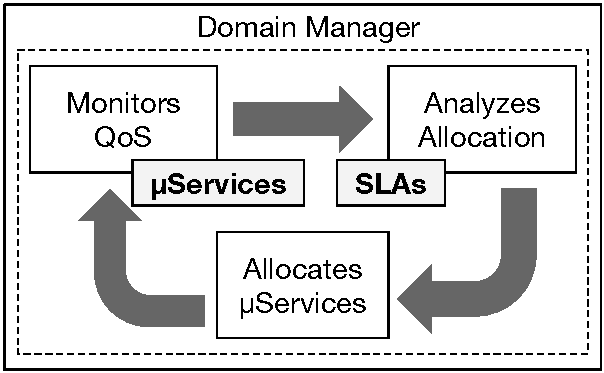
\includegraphics[width=0.4\textwidth]{figs/service-allocation-loop}}
%	\captionsetup[subfigure]{width=0.4\textwidth}	
%	\hfill
%	\subfloat[Per $\mu$-service domain selection control loop; clients monitor $\mu$-services from available domains and select the one that best satisfies its requirements.\label{fig:domain-selection-loop}] {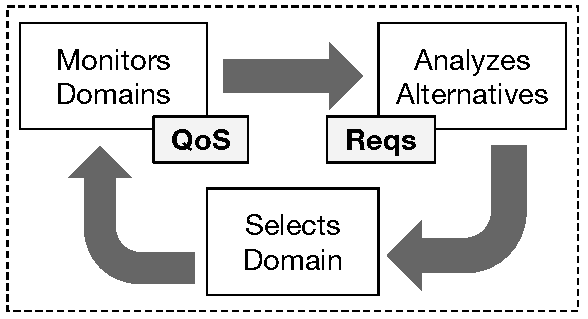
\includegraphics[width=0.4\textwidth]{figs/domain-selection-loop}}
%	\hfill\null
%	\caption{Self-management loops for domain-side $\mu$-services allocation and client-side domain selection}\label{fig:allocation-loops}
%\end{figure}


The \textit{Allocation} models the deployment of continuum $\mu$-services on a pool of resources from cloud and edge domains ($\mu$-services from mobile domains are pre-allocated). It also captures the client-side selection of domains for each of the $\mu$-services employed by the application.

%From the domain's perspective, the allocation phase models the placement of $\mu$-services on the domain's resources, i.e., on its pool of servers, virtual machines, and containers. At the beginning of this phase, $\mu$-service artifacts have been \textit{acquired} by the domain, and the client has been \textit{notified} of this.

The scope of the provider-side Allocation is limited by its domain boundaries. For example, cloud domains allocate $\mu$-services to containers in resourceful datacenters covering a large area. On the other hand, edge domains rely on containers from one or more (virtual) machines serving an office or a building (local-edge) or a 5G base station area (mobile-edge). %In this paper, we do not consider inter-domain cooperation (e.g., placement among different domains).

Existing FaaS platforms handle Allocation with on demand instantiation of containers, which may be kept \textit{warm} before been deallocated after a period of idleness~\cite{AWSLambda, OpenWhisk}. This mechanism can be generalized as a self-management loop~\cite{kephart2003vision} in which the domain manager allocates $\mu$-service instances to guarantee that latency and availability of each provided $\mu$-service cope with its SLA. 


Throughout provider-side Allocation, a \textit{$\mu$-service acquired} event indicates that function(s) and dependencies have been fetched and the $\mu$-service is ready to be deployed. The domain manager must react by including this $\mu$-service in its self-management loop. To mitigate cold start, the manager should react to a \textit{client arrived} event with the anticipation of Allocation upon availability of resources. Finally, a \textit{$\mu$-service requested} event related should be taken into account by by the self-management loop handling Allocation with the increase of the corresponding arrival rate.



%the domain manager deals with the following events:
%{\small
%	\begin{itemize}[noitemsep,topsep=4pt]
%		
%		\item \textbf{$\mu$-service acquired:} indicates that function(s) and dependencies have been fetched and the $\mu$-service is ready to be deployed. The domain manager must react by including this $\mu$-service in its self-management loop handling Allocation.
%		
%		\item \textbf{Client arrived:} indicates the arrival of a client from a given $\mu$-service. To mitigate cold start, the manager should anticipate Allocation upon availability of resources.
%		
%		\item \textbf{$\mu$-service requested}: as defined in Section~\ref{sec:A3-E-engagement}. It should be taken into account by by the self-management loop handling Allocation with the increase of arrival rate ($\lambda_j$).
%		
%	\end{itemize}
%}%


%Traditionally, cloud domains employ automated scaling mechanisms in which virtual machines and container instances are (de)allocated on demand. More recently, cloud-based FaaS platforms (e.g., Amazon Lambda, Google Cloud Functions) extend these mechanisms to stateless functions. The later represent an extreme type of allocation in which no pre-allocation of resources is needed and functions are executed by a shared runtime platform. 

%To realize this activity, the domain manager exploits a self-management control loop~\cite{kephart2003vision} (see Figure~\ref{fig:service-allocation-loop}) in which the $\mu$-services are instantiated according to: (i) a monitored QoS (e.g., the latency with each domain), (ii) a SLA, and (iii) the availability of the computational resources. 
%Once , the DSM informs the client whether the $\mu$-services can be considered ``acquired'' or not.
%For instance, in a centralized implementation, the DSM orchestrates the placement of functions to containers distributed along multiple servers.


%TODO the SLA part is too vague, we must be more assertive regarding priority
%While in cloud domains scalability is virtually unlimited, in finely distributed edge domains scalability needs to be prioritized to favor applications with more demanding requirements. For instance, edge providers could support two types of SLAs: one for critical applications requiring high availability, and another for non-critical applications that may cope with lower degrees of availability.  

%The first type could be achieved with the pre-allocation of resources to these services, whilst the latter could rely on the opportunistic allocation of services upon demand and availability of resources. 
%In the scenario introduced in Section~\ref{sec:continuum}, the AV application should have a higher priority with respect to non-critical applications such as AR applications for tourists~\cite{GarrigaMendonca2017}. In this case the edge $\mu$-services might become unavailable to the AR applications, for example during rush hour. In that case the AR and other low-priority applications would have to rely on $\mu$-services being run in the mobile domain, or in a cloud domain.

%The specific algorithms for the placement of services among the domain's resources that should be employed at the analysis phase are out of the scope of this paper. Nonetheless, recent works~\cite{} have addressed this challenge in the context of a continuum formed by edge and cloud datacenters. 

%Given the state of different domains perceived by a client, the mobile middleware must decide which domain is responsible for each $\mu$-service consumed by the application. 

A self-management loop is also exploited by the mobile middleware in the selection of the domain alternative that best satisfies the client's needs. For each $\mu$-service consumed by the client application, the middleware checks the corresponding QoS levels from the list of domains currently available. %A multi-attribute analysis then decides for the best alternative satisfying the application requirements.
Throughout this activity, the \textit{domain acquired/lost} event indicates the agreement(denial) of a domain in providing a given $\mu$-service. The middleware must react by including(disregarding) this domain in its self-management loop. %Conversely, a \textit{domain lost} event indicates a domain can no longer provide a $\mu$-service. The middleware must react by disregarding this domain in its self-management loop.

Given the resource limitations of edge domains, contention between different $\mu$-services may exist. If we go back to our running example,
% in Section~\ref{sub:example}
critical applications should have a higher priority with respect to others like the AR for tourists. In such cases, edge-based $\mu$-services might become unavailable (or available with an higher response time) to the AR applications. Accordingly, the AR and other low-priority applications could have to rely on $\mu$-services from their own mobile domain or a cloud domain --- as decided by their self-management loop for domain selection. 

%
%{\small
%	\begin{itemize}[noitemsep,topsep=4pt]
%		
%		\item \textbf{Domain acquired:} indicates the agreement of a domain in providing a given $\mu$-service. The mobile middleware must react by including this domain in its self-management loop.	
%		
%		\item \textbf{Domain lost:} indicates a domain can no longer provide a given $\mu$-service. The mobile middleware must react by removing this domain from its self-management loop.
%		
%	\end{itemize}
%}%



%, i.e., it models the computation placement along the client's perception of the continuum. 
%This decision should consider a list of available domains providing services requested by the client application with accompanying QoS attributes. Accordingly, whereas the domains should take care of intra-domain allocation through service placement, the clients are responsible for the inter-domain allocation through service selection.

%Analogously to the domain-side, the CSM manages allocation with a self-management loop , this time by checking QoS levels of services from each available domain and deciding for the alternative that best satisfies the client's requirements. 

%This sub-process is the main client-side activity required for the realization of the continuum, as it allows clients to seamlessly alternate among different continuum domains according to the context. 

%TODO [Danilo] check the consistency of the usage of the running example in this Section
%If we go back to our running example, in the absence of appropriate edge domains, the low-priority AR applications would need to choose between their local mobile domain and the cloud domain. If the application's requirements favor low-battery consumption, the cloud domain will be chosen for allocation. Otherwise, if low latency is the most important QoS metric, the local mobile domain will be chosen. As the number of requirements grows, a multi-objective optimization algorithm may be employed to decide among alternative domains.


%, upon unavailability of edge domains providing services with low latency, the AR application previously introduced would have to choose among mobile or cloud domain. If the application requirements prioritizes low battery consumption (e.g., because battery level is low), it should opt for the cloud domain. Otherwise, if low latency is the priority requirement, it should opt for the cloud domain. 



%The allocation phase has the following purposes: 1) to enable the efficient (Req. \textbf{R1.1}) and automated (Req. \textbf{R3.1}) allocation of domains' computational resources; and to enable clients to choose the best candidate among different available domains (Req. \textbf{R2.1}).

\subsection{Engagement}\label{sec:A3-E-engagement}

A3-E's \textit{Engagement} models the actual provisioning of a continuum $\mu$-service by a domain after its successful allocation.
%: at the beginning of this phase, the continuum $\mu$-service has been \textit{allocated} by a domain, which in turn has been previously \textit{selected} by the client. 
Throughout this activity and as long as the client-domain relation persists, the client is able to engage with that domain by means of invocations to the provided $\mu$-service. 

Remote domains (i.e., cloud and edge) are engaged through distributed protocols (e.g., HTTP requests or WebSockets). To enforce a common interface between the mobile middleware and heterogeneous domains, the mobile domain should also expose its functionality as local services decoupled from the client application.

During Engagement, a \textit{$\mu$-service deallocated} indicates the unavailability of a given $\mu$-service. The manager must react by queuing or sending a \textit{request response} signal with error code to subsequent requests. Conversely, a \textit{$\mu$-service allocated} indicates the availability of a given $\mu$-service. The manager must react by resuming the processing of queued and subsequent requests. Finally, the manager must handle a \textit{$\mu$-service requested} with the placement of the request to a service instance after a \textit{load balancing} strategy.

%indicates the arrival of a request for a specific $\mu$-service. The manager must handle the event with the placement of the request to a service instance after a \textit{load balancing} strategy.

%the domain manager deals with the following events:
%
%{\small
%	\begin{itemize}[noitemsep,topsep=4pt]
%		
%		\item \textbf{$\mu$-service deallocated:} indicates the unavailability of a given $\mu$-service. The manager must react by queuing or sending a \textit{request response} signal with error code to subsequent requests.
%		
%		\item \textbf{$\mu$-service allocated:} indicates the availability of a given $\mu$-service. The manager must react by resuming the processing of queued and subsequent requests.	
%		
%		\item \textbf{$\mu$-service requested:} indicates the arrival of a request for a specific $\mu$-service. The manager must handle the event with the placement of the request to a service instance after a \textit{load balancing} strategy.
%	\end{itemize}
%}%

From the client's viewpoint, a \textit{C-request arrived} indicates the client application has sent a new request to a continuum $\mu$-service. The event contains the target $\mu$-service reference along with any parameters. The middleware must handle it by invoking the $\mu$-service from the currently selected domain. Upon arrival of a \textit{request served}, the middleware must proceed with the triggering of a \textit{C-Request served} event to be handled by the client application. 

Also during this activity, a \textit{domain absent} event indicates no domain is available for that specific $\mu$-service. The middleware must react by queuing subsequent C-requests and, in case of latency violation, firing a \textit{C-request failed} event. In turn, a \textit{domain changed} event indicates a new domain selection for a specific $\mu$-service. The middleware must handle it by resuming the invocation of any queued and subsequent C-requests to that domain.

%
%The mobile middleware deals with the following events:
%
%{\small
%	\begin{itemize}[noitemsep,topsep=4pt]
%		
%		\item \textbf{C-Request arrived:} indicates the client application has sent a new request to a continuum $\mu$-service. The event contains the target $\mu$-service reference along with any parameters. The middleware must handle it by invoking the $\mu$-service from the currently selected domain.
%		
%		\item \textbf{Request served:} indicates the arrival of a response from a domain for an invoked service. The middleware must handle it with the triggering of a \textit{C-Request served} event to be handled by the client application.
%		
%		%\item \textbf{C-Request served:} indicates a given C-request has been processed. It contains the original $\mu$-service reference along with any return value(s). The client application is responsible for handling the event.	
%		
%		\item \textbf{Domain changed:} indicates a domain have been selected for a specific $\mu$-service. The middleware must handle it by resuming the invocation of any queued and subsequent C-requests to that domain.
%		
%		\item \textbf{Domain absent:} indicates no domain is available for that specific $\mu$-service. The middleware must react by queuing subsequent C-requests and, in case of latency violation, firing a \textit{C-request failed} event.
%		
%	\end{itemize}
%}%

%TODO [Danilo] requirements must be passed by the application before, otherwise the domain selection would need to happen after the request has been fired
%It also contains continuum requirements that must be taken into account by the middleware in the decision of which 

%Two types of event dictate the end of an engagement: i) the client makes no further requests after a time interval; ii) the client selects another domain; and iii) the domain manager requires the deallocation of the service instance. 

%In all three cases, resources become available in the domain. In the latter case, the client is forced to select another domain.


%In this phase the request has already been provisioned by one or more domains and the client-side middleware (CSM) has already selected a specific domain to make the request. 

%handled and parsed by the client-side middleware (CSM), and . 


%Also, one or more domains must have setup and allocated the requested service for execution and the CSM must have selected a specific domain among all providing the same service. Finally, client's request are sent, processed, received, and returned to the application.

%Current FaaS providers allow functions to be exposed as REST services. The same applies to open source platforms implementing the FaaS model. Finally, different approaches may be used to expose local computation as services in mobile platforms like Android and iOS.

%As an exception, computation provided by mobile devices can be accessed by means of local calls to functions executed by the mobile platform.

%%What: how different policies may be employed by domains and clients throughout A3-E-Process
\subsection{A3-E Process: Domain Policies}\label{sec:A3-E-policies}

\begin{figure}[tbp]
	\raggedright
	\subfloat[Different states of a given edge domain with respect to a given client application; the transitions between states triggered by domain events are guarded by policies that may vary according to the type of domain and the SLA with different applications\label{fig:A3-E-domain}] {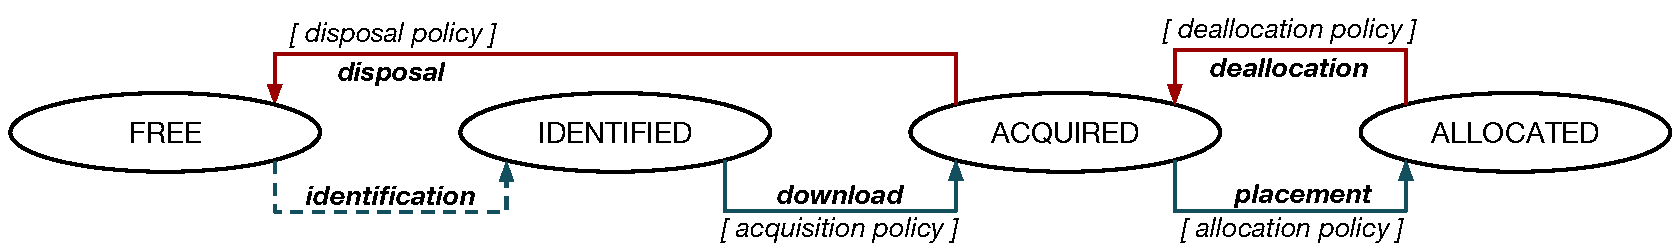
\includegraphics[width=0.95\textwidth]{figs/A3-E-domain}}\hfill
	
	\subfloat[Different states of a given client with respect to a given edge domain; the transitions between states triggered by client events are guarded by policies that may vary according to the client requirements\label{fig:A3-E-client}] {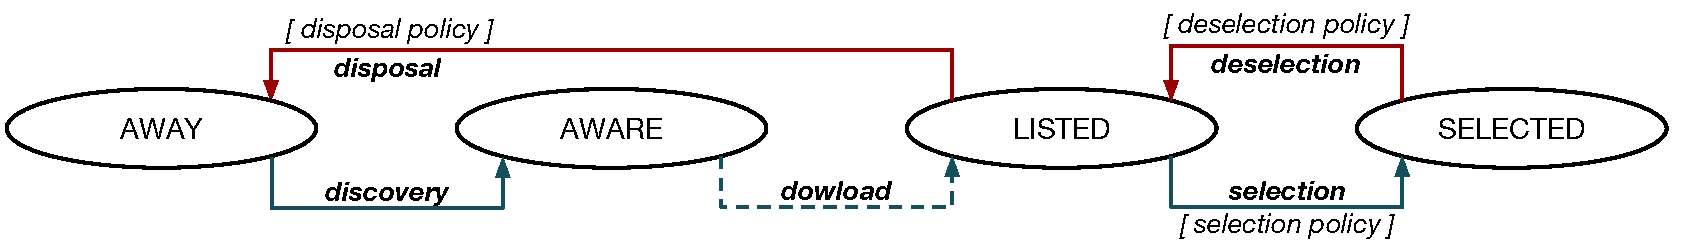
\includegraphics[width=0.95\textwidth]{figs/A3-E-client}}\hfill
	\caption{States and transitions among A3-E phases} \label{fig:A3-E-states}
\end{figure}


%What: the flexibility of A3-E model in terms of policies that regulate the transition among phases

The A3-E process is also flexible with respect to the transitions among subsequent phases. In particular, distinct policies may define different behaviors for the transition. Figures~\ref{fig:A3-E-domain} and~\ref{fig:A3-E-client} depict, respectively, the possible transitions among states of a domain with respect to a client application and vice-versa. Each state is mapped to the corresponding phase in Fig.~\ref{fig:A3-E-model}. 

From the domain perspective, policies affect the following conflicting properties: a) the \textit{efficiency} of domain resource usage; and b) the service setup \textit{delay}. Considering the first request arrival ($FRA$) from a client application as the reference event, the more \textit{reactive} the policies are to that event, the less time domain resources are likely to remain idle before it happens (more efficiency). In contrast, the chances of underutilization and idleness are higher with \textit{proactive} policies (less efficiency). Eq.~\ref{eq:setup_cost} models the total delay of service setup:

\begin{equation}\label{eq:setup_cost}
C_{SETUP} = C_{OFFLINE} + C_{RUNTIME}
\end{equation}

\noindent
in which the first term ($C_{OFFLINE}$) represents the resources required for downloading and installing the services (e.g., network and storage), whilst the later ($C_{RUNTIME}$) represents the resources needed for executing the services (e.g., memory and CPU). 

From the delay point of view, the relation is the opposite: the more \textit{reactive} the policies are with respect to the first request arrival event, the higher the delay the first request to each service is served with. In the other direction, the more \textit{pro-actively} services are made ready for execution, the lower the delay the first request to each of these services is served with. Eq.~\ref{eq:setup_delay} models the total delay of service setup:

%\Delta_{NET} + 
\begin{equation}\label{eq:setup_delay}
L_{SETUP} = \Delta_{AW} + \Delta_{AQ} + \Delta_{AL}
\end{equation}

\noindent
in which the first term ($\Delta_{AW}$) represents the time it takes for clients and domains to become aware of each other. The second term ($\Delta_{AQ}$) represents the time for acquiring all assets of a specific service, whilst the last term ($\Delta_{AL}$) represents the time for allocating resources for the service execution. 

For instance, existing cloud-based FaaS platforms (e.g., Amazon Lambda, Google Cloud Functions, and Apache OpenWhisk) employ on demand allocation of stateless functions, i.e., functions are reactively allocated upon arrival of the first request. Depending on the policy configuration, the platform waits for an idleness interval before deallocating the function~\footnote{\url{https://read.acloud.guru/how-long-does-aws-lambda-keep-your-idle-functions-around-before-a-cold-start-bf715d3b810}}. In these cases, the improved efficiency of the platform in allocating computational resources has the drawback of a setup delay (cold start). 

The domain-side policies in Fig.~\ref{fig:A3-E-domain} can be refined into three types: \textit{proactive} (P), \textit{sequential} (S), and \textit{reactive} (R). 

\begin{itemize}

\item \textbf{Proactive}: acquisition phase starts upon external event preceding the $FR_A$ event (e.g., the prediction of service usage in the near-future). Benefits: first response delay ($FR_D$) does not include $\Delta_{AQ}$. Drawback: acquired artifacts remain idle until usage. Example: stateless functions required by body device applications during a marathon event are fetched the night before the event by mobile-edge domains located along the course. 

\item \textbf{Sequential}: the beginning of acquisition phase is dictated by the completion of the awareness phase. Benefits: service artifacts are only acquired upon detection of a potential client in the domain coverage area, minimizing the likelihood of idleness. Drawbacks: $FR_D$ may include a fraction of $\Delta_{AQ}$ if $FRA$ precedes the end of acquisition. Example: stateless functions to be consumed by a mobile multiplayer game application are acquired by an indoor-edge domain inside a passenger train upon detection of two or more clients in the train.

\item \textbf{Reactive}: acquisition phase starts upon detection of a $FRA$. Benefits: acquisition of service artifacts follows an actual demand, eliminating artifacts storage idleness. Drawbacks: $FR_D$ includes $\Delta_{AQ}$, which may be disruptive for some applications. Example: stateless functions to be consumed by a TODO 

%the notion of a reactive allocation can be extended also to the acquisition of service artifacts. Instead of having functions pre-downloaded and installed, this process could happen in reaction to the first arrival of a request. 

\end{itemize}

In turn, the allocation phase can be triggered according to the following policies:

%The \textit{allocation policies} in Fig.~\ref{fig:A3-E-domain} can be:

\begin{itemize}

\item \textbf{Proactive}: allocation phase starts upon external event preceding the arrival of the first request (e.g., the prediction of service usage in the near-future). Benefits: $FR_D$ does not include $\Delta_{AL}$. Drawback: allocated resources remain idle until $FR_A$. Example: stateless functions to be consumed by connected vehicles are pre-allocated by mobile-edge domains in specific day times.

\item \textbf{Sequential}: allocation phase starts as soon as acquisition phase finishes. Benefits: depends on the acquisition policy. Drawbacks: depends on the acquisition policy. Example: stateless functions required by a marathon application running on body devices are allocated following their acquisition by the mobile-edge domains along the course.

\item \textbf{Reactive}: allocation phase starts as soon as $FR_A$ is detected. Benefits: eliminates idleness by conditioning allocation to an actual service demand. Drawback: $FR_D$ includes $\Delta_{AL}$ (cold start). Example: stateless functions required by a mobile multiplayer game are allocated by a local-edge domain inside a train following the detection of a $FR_A$ event.

\end{itemize}

%
%\begin{itemize}
%	
%	\item \textbf{Proactive}: . Benefits: . Drawback: . Example: .
%	
%	\item \textbf{Reactive}: . Benefits: . Drawback: . Example: .
%	
%\end{itemize}
%
%
%\begin{itemize}
%	
%	\item \textbf{Proactive}: . Benefits: . Drawback: . Example: .
%	
%	\item \textbf{Reactive}: . Benefits: . Drawback: . Example: .
%	
%\end{itemize}
%
%
%\subsubsection{Client-Side Policies}
%
%Clients may also adopt different policies for the selection and deselection of domains (Fig.~\ref{fig:A3-E-client}), namely:
%
%%domains are selected based on their category (cloud, edge, local) or/and 
%
%\begin{itemize}
%	
%	\item \textit{Selection policy}
%	
%	\begin{itemize}
%		
%		\item \textbf{Proactive}: 
%		
%		\item \textbf{Reactive}: 
%		
%	\end{itemize}
%	
%	\item \textit{Deselection policy}
%	
%	\begin{itemize}
%		
%		\item \textbf{Proactive}: 
%		
%		\item \textbf{Reactive}: 
%		
%	\end{itemize}
%\end{itemize}


%
%\subsection{Reference Architecture}
%
%\begin{figure}[tbp]
%	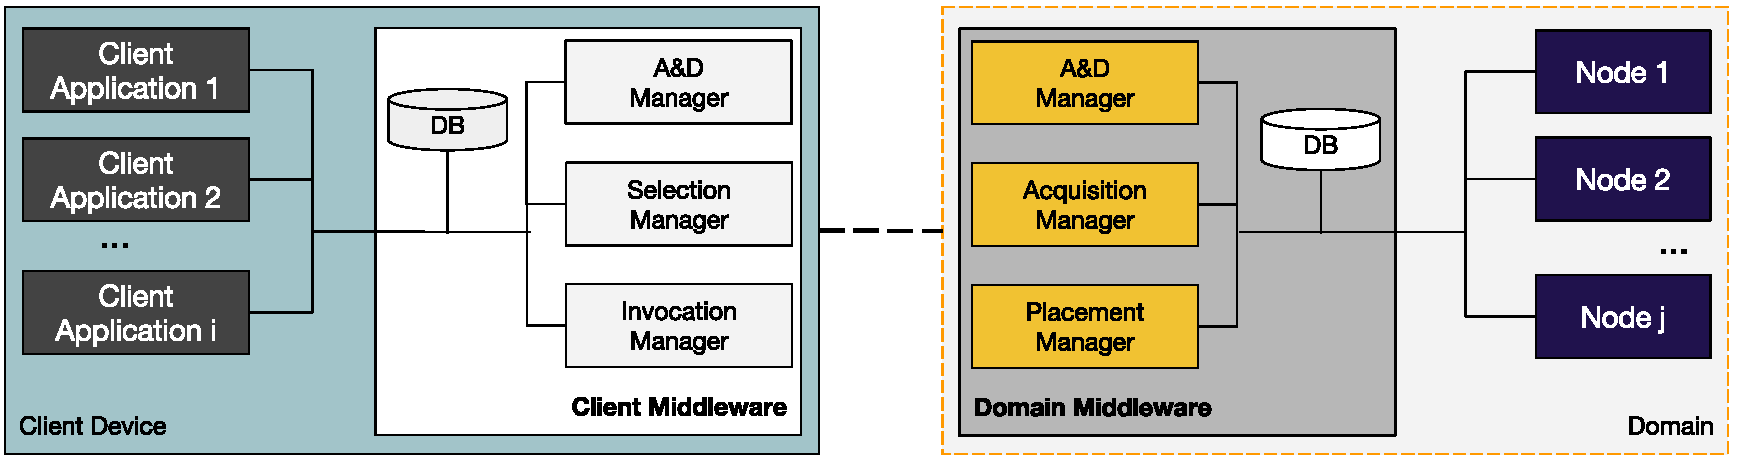
\includegraphics[width=.95\textwidth]{figs/A3-E-reference-architecture}
%	\caption{A3-E architecture in Mobile Devices and edge domains}
%	\label{fig:reference-architecture}
%	\end{figure}
